\documentclass[10pt,twocolumn,letterpaper]{article}

\usepackage{cvpr}
\usepackage{times}
\usepackage{epsfig}
\usepackage{graphicx}
\usepackage{amsmath}
\usepackage{amssymb}

% Include other packages here, before hyperref.

% If you comment hyperref and then uncomment it, you should delete
% egpaper.aux before re-running latex.  (Or just hit 'q' on the first latex
% run, let it finish, and you should be clear).
\usepackage[breaklinks=true,bookmarks=false]{hyperref}

\cvprfinalcopy % *** Uncomment this line for the final submission

\def\cvprPaperID{****} % *** Enter the CVPR Paper ID here
\def\httilde{\mbox{\tt\raisebox{-.5ex}{\symbol{126}}}}

% Pages are numbered in submission mode, and unnumbered in camera-ready
%\ifcvprfinal\pagestyle{empty}\fi
\setcounter{page}{1}
\begin{document}

%%%%%%%%% TITLE
\title{Generating Novel Works of Art Using Generative Adversarial Networks}

\author{Bradley Beyers\\
	University of Rochester\\
	{\tt\small bbeyers@u.rochester.edu}
	% For a paper whose authors are all at the same institution,
	% omit the following lines up until the closing ``}''.
	% Additional authors and addresses can be added with ``\and'',
	% just like the second author.
	% To save space, use either the email address or home page, not both
	\and
	Santiago Loane\\
	University of Rochester\\
	{\tt\small sloane@u.rochester.edu}
}


\maketitle
%\thispagestyle{empty}

%%%%%%%%% ABSTRACT
\begin{abstract}
   In this work, we explore the applicability of Generative Adversarial Networks (GANs)
   to the task of generating novel works of art. Utilizing a variant of the Deep Convolutional GAN (DCGAN)
   architecture \cite{radford2015unsupervised}, we train generative models on a dataset of 203,275 visual works of art. We show empirically that the DCGAN architecture is able to learn and reproduce salient features of visual artwork such as color, shape, composition and style. We also show several pieces of evidence that our models have learned semantically meaningful and artistically useful representations.
\end{abstract}

%%%%%%%%% BODY TEXT
\section{Introduction}
The comprehension and production of artwork is considered by many to involve skills available
uniquely to humans. Human artists incorporate a wealth of cultural knowledge, personal experiences,
and creativity in their work. A model which could produce output human observers would accept
as novel works of art could be said to possess some representation of the artistic knowledge
that humans tap into when they create art. By examining these learned representations, we can
learn more about what they are able to encode and how they are able to encode it. In the case of convolutional neural networks, whose architecture is designed to roughly mirror the structures of neurons that make up our brains, analysis of the representations learned by such a model may even yield some insight into the way humans process visual information.

The computer-based generation of images which appear natural has in the past been limited to
the rendering of images based on models and textures carefully designed by humans. More recently, new techniques have surfaced to create models capable of generating realistic images automatically such as Variational Auto-Encoders \cite{kingma2013auto, kingma2014semi} and auto-regressive models \cite{larochelle2011neural, germain2015made}. Deep learning has also opened up the possibility of realistic image generation through the use of neural networks. Goodfellow \etal \cite{goodfellow2014generative} introduced Generative Adversarial Networks
(GANs), a framework for training generative models using backpropagation which has recently become popular for training models capable of generating images\cite{huang2017stacked, denton2015deep, reed2016generative}. Radford \etal \cite{radford2015unsupervised} present techniques for the effective training of Deep Convolutional GANs (DCGANs), or deep convolutional neural networks within the GAN framework, which have remained popular since their introduction \cite{gulrajani2017improved, reed2016generative, arjovsky2017wasserstein}.

By training a DCGAN on a dataset of visual works of art, we create models which can generate images
which capture salient properties of artwork produced by human artists. We empirically assess the
quality of samples generated by our model and discuss the features it was able to learn.
Using analysis techniques discussed by Radford \etal \cite{radford2015unsupervised} as well as 'deconvnets' first discussed by Zeiler \cite{zeiler2011adaptive} then improved by Zeiler and Fergus \cite{zeiler2014visualizing}, we investigate the representations learned by our model more directly.

\section{Related Work}
\subsection{Generative Adversarial Networks}
First proposed by Goodfellow \etal \cite{goodfellow2014generative}, GANs are a general
framework which may be used to learn generative models of data distributions. In GANs, two models
are employed, a discriminator $ D $ and a generator $ G $. $ G $'s goal is to produce output
which mimics the features of some known data distribution $ p_{data} $, and $ D $'s goal is to distinguish
real samples drawn from $ p_{data} $ from fake samples generated by $ G $. To produce its output, $ G $
takes as input a sample $ z $ from a noise distribution $ p_{z} $. Formally, $ D $ and $ G $ play
a minimax game whose value function is defined as

\begin{equation}
\begin{aligned}
\min_{G} \max_{D}  & \mathbb{E}_{x \sim p_{data}(x)}[log(D(x))]	+ \\
				   & \mathbb{E}_{z \sim p_{z}}[log(D(G(z)))].
\end{aligned}
\end{equation}

In other words, $ D $ attempts to maximize its chances of correctly correctly classifying its input
as real or fake, and $ G $ attempts to minimize $ D $'s chances of doing so. If suitable choices
are made for the model architecture of $ D $ and $ G $, GANs may be trained using backpropagation.

\subsection{Deep Convolutional Generative Adversarial Networks}
Goodfellow \etal \cite{goodfellow2014generative} explored the potential for convolutional neural
networks in a GAN framework to learn a generative model of the well-known CIFAR-10 dataset
\cite{krizhevsky2014cifar}. Radford \etal \cite{radford2015unsupervised} expand on this idea,
introducing DCGANs. Their results include a set of guidelines for effective training of
DCGANs. They suggest replacing downsampling and upsampling layers with convolution and transpose
convolution layers respectively so that the networks can learn their own down- and upsampling. Additionally, they recommend the use of batch normalization to stabilize the training process, and the LeakyReLU activation function \cite{maas2013rectifier} to help speed up training in the discriminator network.

\subsection{Network Analysis Methods}
Radford \etal also discuss several methods of investigating the representations learned by the generator
network of a DCGAN. One method is walking through the latent space of $ G $'s input. If $ G $ has managed
to learn relevant and meaningful features of $ p_{data} $, then walking through the latent space will
yield smooth transitions between semantic concepts in $ G $'s output space. On the other hand, sharp, sudden changes in the output space while moving smoothly in the input space may be a sign that the model is memorizing input data, or collapsing entire regions of its input space to the same point in output space, which may indicate a failure to learn meaningful, useful representations.

Another is searching for evidence that vector arithmetic in $ G $'s input space can result in meaningful
manipulation of the features of its output. This was first demonstrated by Mikolov \etal in 2013 \cite{mikolov2013distributed} where learned vector representations of words were found to have useful semantic structure. For example, if $ K $ is the vector that represents the word "King", $ M $ is the vector for "Man" and $ W $ is the vector for "Woman", then $ K - M + W $ would give a vector near the vector for "Queen," logically combining the semantic properties of the vectors involved. Radford \etal \cite{radford2015unsupervised} show the presence of similar structure in their generator network's input space, allowing them to manipulate its output in meaningful ways, like adding sunglasses to an image of a person's face.

'Deconvnets' or deconvolutional networks, first introduced by Zeiler \cite{zeiler2011adaptive} then improved by Zeiler and Fergus \cite{zeiler2014visualizing}, are a technique for visualizing the representations learned by convolution layers in convolutional neural networks. Deconvnets approach the problem of visualizing the concepts learned by high-level convolution layers by taking a fully trained convolutional neural network and a choosing a single neuron in a higher layer. An image is passed forward through the network, and then the activations of all neurons other than the target neuron are set to 0. Then, the activation is passed backward through a deconvnet, which reconstructs the activations of the layers preceding that of the target neuron. This progressive reconstruction will eventually reach the input layer, where it will reconstruct the pattern of pixels which caused the activation of the target neuron. By visualizing the reconstructed activations of the intermediate layers and input layer, we can get a sense of the features each neuron in the network examines, as well as the patters in input which tend to activate a particular high-level neuron.

\section{Methods}
\subsection{Data}
Before attempting to train a DCGAN on a dataset of artwork, we first validated the architecture of our models by training them on the well-known MNIST dataset of handwritten digits \cite{lecun2010mnist}. The advantage to training on MNIST is that the visual features of a well-formed digit are simple and obvious, whereas the visual features of a well-formed painting are difficult to concretely define. As a result, training models on MNIST serves as a useful proof-of-concept, since visual inspection of a model's output can more easily verify whether it is able to learn useful features of the dataset. To conduct our experiments on artwork, we compiled images of visual works of art from two sources, Kaggle and Wikiart.

Kaggle is a platform for hosting data science and machine learning competitions in which teams compete to complete a task defined by those hosting the competition. The Kaggle "Painter By Numbers" competition challenged competitors to predict whether pairs of paintings were created by the same artist. The accompanying dataset contains 79,420 images labeled with a hash of the artist's name, the title of the work, the style, the genre, and the date it was created.

Wikiart is an online encyclopedia of visual artwork maintained by users in a manner similar to Wikipedia. On their "About" page, Wikiart claims to host around 250,000 pieces of artwork from around 3,000 artists. Using a script to scrape images from their site, we were able to gather 123,854 images of paintings and some other kinds of visual artwork. Most, but not all of the images contain most of the same metadata as the Kaggle dataset. 98.29\% of images are labeled with their artist, 95.14\% are labeled with their genre, and 94.57\% are labeled with their style.

Combining these two sets of data, we managed to assemble a dataset of 203,274 paintings and other works of visual artwork. Each image was resized, maintaining its aspect ratio, so that it was the smallest possible size that still had at least $ 16,384 $ pixels (such that a square image would be $ 128 \times 128 $). During training, a random $ 64 \times 64 $ patch of the image is used as the training data. This has several advantages. For one, resizing the dataset drastically reduces its overall size. Using a random patch of the image also serves to augment our training data since many different patches from the same image may be used throughout training, which helps combat overfitting. Finally, the this technique allows our training data to maintain its original aspect ratio while resizing it so that it can be used as input for $ D $. Changing the aspect ratio would warp features of the input, potentially resulting in less effective training.

\subsection{Model Construction}
The model architecture we used for our experiments is based on the model architecture for DCGANs presented by Radford \etal in \cite{radford2015unsupervised}. The discriminator network consists of a series of 4 convolution layers with a fully connected layer at the end. Each convolution layer has a $ 4 \times 4 $ kernel, a stride of 2, and padding of 1. After every convolution layer but the first, we apply batch normalization, and every convolution layer uses the Leaky ReLU activation function \cite{maas2013rectifier} with a leak coefficient of $ 0.2 $. The depth of the feature map increases with each convolution layer. Starting from the 3 channels of the input, the first convolution layer has 128 filters, the second has 256, the third has 512 and the final has 1024. The final fully connected layer uses the sigmoid activation function to compute the final output of the network.

The architecture of the generator network is similar to the discriminator network in reverse. It progressively upscales its input and makes it shallower through a series of 5 transposed convolution layers, sometimes called "deconvolution" layers. The first layer has 1024 filters, a $ 4 \times 4 $ kernel, a stride of 1 and no padding. Its purpose is to take a noise vector and use it to generate a high-level feature map of the output image. The remaining 4 transpose convolution layers have 512, 256, 128, and 3 filters respectively, and each has a $ 4 \times 4 $ kernel, a stride of 2 and padding of 1. Mirroring the discriminator, each of the first 4 transpose convolution layers is followed by batch normalization and the Leaky ReLU activation function \cite{maas2013rectifier} with a leak coefficient of $ 0.2 $. The final transpose convolution layer uses the $ \tanh $ activation function.

\begin{figure}[t]
	\begin{center}
		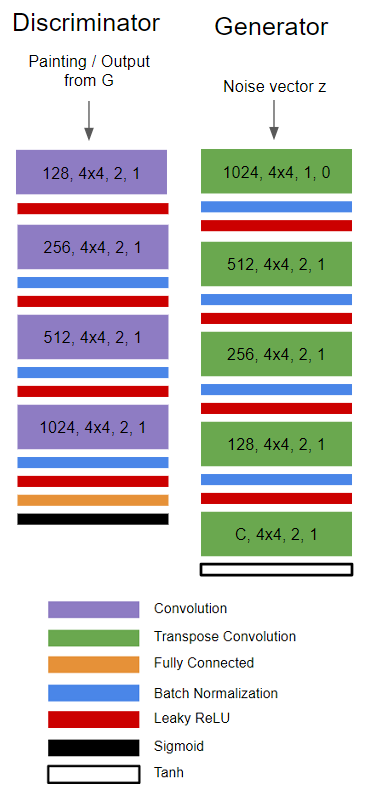
\includegraphics[width=0.8\linewidth]{nets1.png}
	\end{center}
	\caption{A diagram representing the network structure of the discriminator and generator. The colored blocks, read top to bottom, describe the sequence of layers in the network and give the parameters of the convolution and transpose convolution layers. Each convolution or transpose convolution layer is labeled with its number of filters, kernel size, stride, and padding.}
	\label{fig:long}
	\label{fig:onecol}
\end{figure}

\section{Experiments}
Our models were constructed and trained using Pytorch \cite{paszke2017automatic}, a Python framework for tensor computation as well as deep learning. We used the same hyperparameters for training in each of our experiments, and both the discriminator and generator networks used the same hyperparameters. We trained our models using the Adam optimization algorithm \cite{kingma2014adam} with a learning rate of $ 10^{-4} $,  $ \epsilon = 10^{-8} $, $ \beta_{1} = .5 $ as suggested by Radford \etal \cite{radford2015unsupervised}, and $ \beta_{2} = .999 $. For all experiments, we used a batch size of 128. The input to the generator network was generated by taking 100 samples from a normal distribution with a mean of 0 and standard deviation of 1, and combining those samples into a 100-dimensional vector.

\subsection{Training on MNIST}
As discussed in section 3.1, we first conducted experiments on the well-known MNIST dataset of handwritten digits. We chose to run experiments on MNIST as a proof-of-concept to validate our model architecture and show that it is able to learn meaningful features of the dataset. Figure 2 shows a collection of 128 output samples generated after 15 epochs of training on MNIST. The samples show that the model was able to learn useful features of handwritten digits, with most samples appearing to be plausible handwritten digits. Some samples, like the ones highlighted in red in figure 2, display ambiguity between classes of digits. While they do have some visual properties of handwritten strokes, they combine features from different digits and as a result do not belong distinctly to any particular class.

\begin{figure}[t]
	\begin{center}
		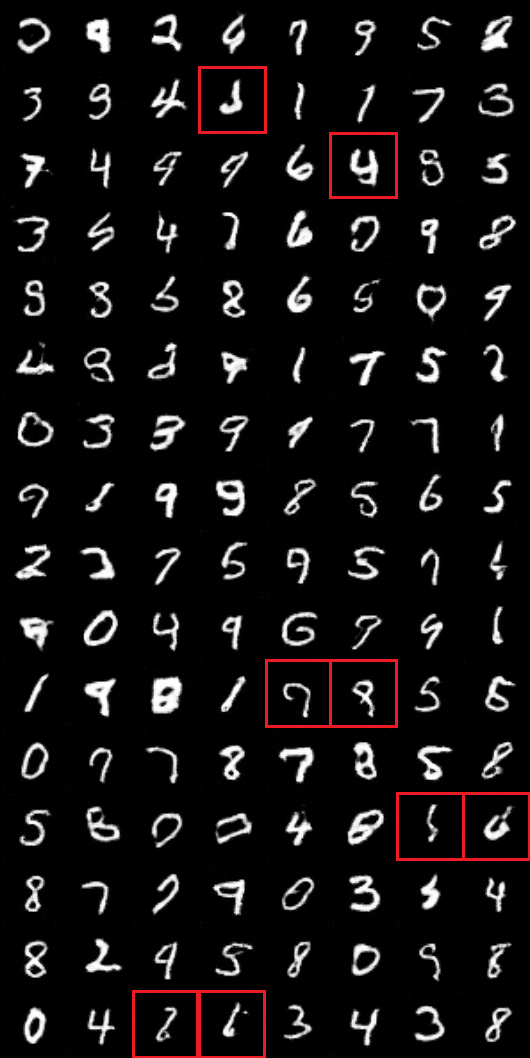
\includegraphics[width=0.775\linewidth]{mnist_samples.png}
	\end{center}
	\caption{Sample output from our network trained on MNIST for 15 epochs. Samples show clear signs that the network has learned salient features of the dataset, and most samples are plausible handwritten digits. Highlighted with red boxes are samples showing ambiguity between classes of digits.}
	\label{fig:long}
	\label{fig:onecol}
\end{figure}

\subsection{Training on Art}
After running experiments on MNIST, we moved on to training our networks on our dataset consisting of 203,274 paintings formed from the combination of the Kaggle "Painter by Numbers" dataset and paintings we were able to scrape from Wikiart. Figure 3 shows a collection of 128 output samples generated by the generator network after 100 epochs of training, which took roughly two days to complete. The samples showcase some of the artistic features our generator network has managed to learn. Most of the samples contain coherent and visually interesting color palettes, and certain samples even contain color palettes which are recognizable as approximations of color palettes found in specific genres of art. Many samples have some semblance of form and shape, although the forms present in the samples are not resolvable as any specific object. Occasionally, our model produces output with a globally cohesive sense of composition, which results in images that have a recognizable genre such as a landscape painting or that appear at a high level to have been created with specific media like watercolor paints or black pencil.

\begin{figure}[t]
	\begin{center}
		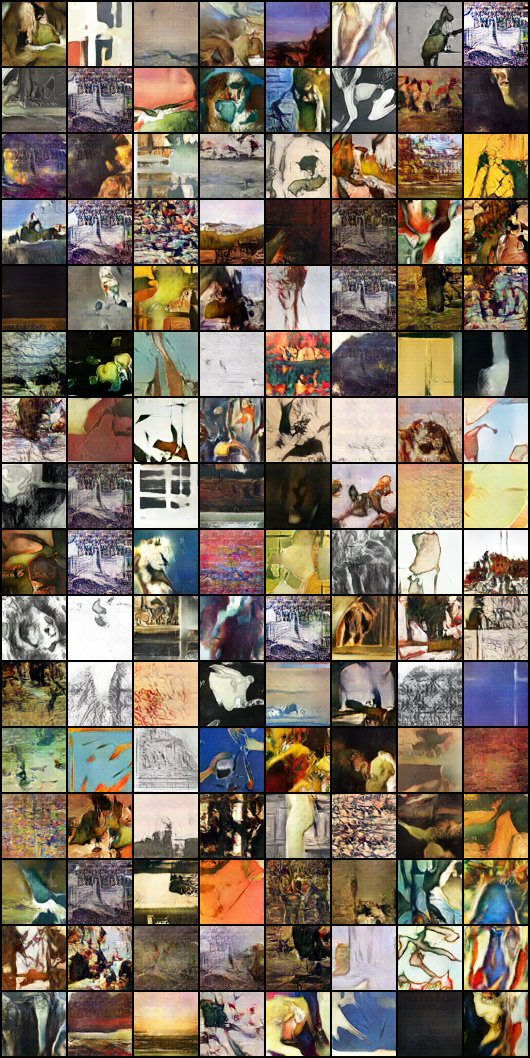
\includegraphics[width=0.775\linewidth]{art_samples.png}
	\end{center}
	\caption{Sample output from our network trained on our art dataset for 100 epochs. Samples show several features which are visually similar to artwork produced by humans such as interesting color palettes, use of shape and form, as well as globally coherent composition in some cases.}
	\label{fig:long}
	\label{fig:onecol}
\end{figure}

\subsection{Learned Representation Analysis}
After fully training our models, we employed the techniques described in section 2.3 to analyze the representations they had learned. 

The first method we used was linear interpolation between points in $ G $'s input space. If $ G $ has learned useful, semantic representations, then smooth interpolation in its input space will yield smooth, meaningful changes in its output space. Figure 4 shows the results of this analysis. Each row from the figure starts with an image generated by $ G $ from a different noise sample. The rest of the row then shows the images generated by $ G $ from the interpolated points moving toward the start of the next row. The bottom row then wraps back around to the top row. We can see that smooth interpolation in our model's input space yields smooth transitions between color palettes, the smooth morphing of the forms in one image to the forms in the next, and even smooth transitions between the style of one image to the next. Altogether, the results of this experiment show strong evidence that our model was able to learn semantically meaningful representations of artistic features.

The second method was vector arithmetic between points in $ G $'s input space. Our approach was to attempt to extract a vector which encodes a specific feature of one image, then use the extracted vector to introduce that feature into a new image. To perform this, we select 3 vectors in $ G $'s input space, $ z_1 $, $ z_2 $ and $ z_3 $. If $ G(z_1) $ is an image with some specific desired property and $ G(z_2) $ is an image which lacks that property, then $ z_1 - z_2 $ should be a vector which encodes that property. Hence $ G(z_1 - z_2 + z_3) $ should be an image similar to $ G(z_3) $, but with the feature encoded by $ z_1 - z_2 $ added to it. Figure 5 shows the results of performing this experiment 3 different times. In each of 5a, 5b and 5c, the first image is $ G(z_1) $, the second is $ G(z_2) $, and each row after the bracket shows the results of a different choice of $ z_3 $. In figure 5a, we selected a $ G(z_1) $ to be a vibrantly colorful image, and $ G(z_2) $ to be a less colorful image. For all of our choices of $ z_3 $, the results turned out colorful, but are all similar and lack meaningful features from $ G(z_3) $. In figure 5b, $ G(z_1) $ is an image that has detailed texture, and $ G(z_2) $ has relatively uniform texture. The results show some limited transfer of textures from $ G(z_1) $ and tend to be less colorful than their corresponding $ G(z_3) $, but do appear to retain some features of $ G(z_3) $ like color in the first and third rows, and shape in the second row. In figure 5c, $ G(z_1) $ is an image that has elements of a landscape painting, and $ G(z_2) $ is an image chosen arbitrarily. The resulting images for each choice of $ z_3 $ show strong transfer of features from $ G(z_1) $ and evidence of features retained from $ G(z_3) $. Overall, these results are mixed. Vector arithmetic does appear to cause changes related to properties of the corresponding images, but the manner in which they are connected is difficult to ascertain because of the dominance of features from $ G(z_1) $.

Our final method was to use a deconvnet to visualize some of the representations learned by $ D $'s convolution layers. These representations are interesting because during training, $ D $ learns on real artwork and samples from $ G $, whereas $ G $ learns only from the signal $ D $ provides. Thus, any representations learned by $ G $ are ultimately derived from those learned by $ D $. Figure 6 shows a sample of the activations recovered from each convolution layer in $ D $ after an example image is passed through them. Detailed features of the input image are clearly visible in the first convolution layer's activations, and some basic shapes are visible in the second layer's activations, showing that $ D $ and by extension $ G $ was able to learn low- and mid-level representations of common artistic features. On the third and final layers, features from the input image are no longer visible, a possible visual indication that the network has processed them into higher-level representations that are no longer human-readable. 

\begin{figure}[t]
	\begin{center}
		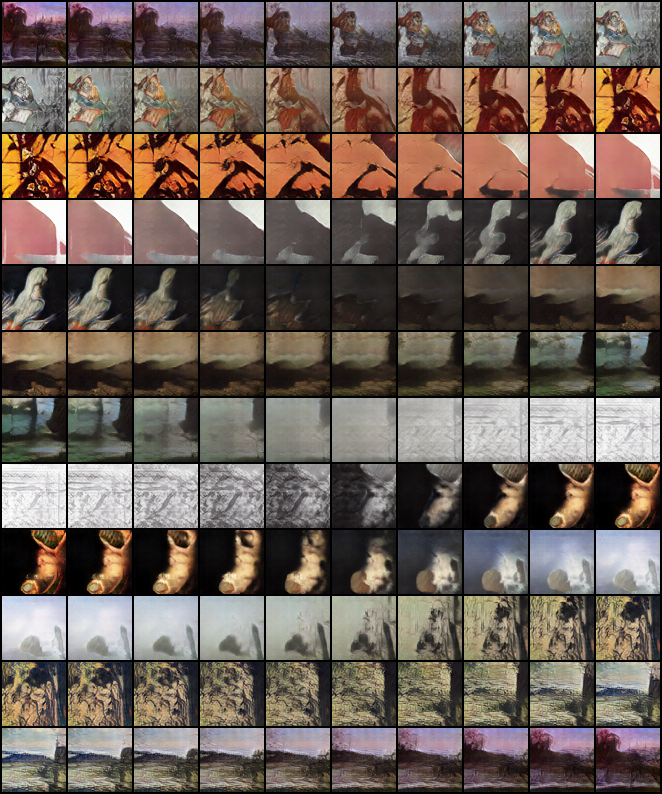
\includegraphics[width=0.9\linewidth]{interp.png}
	\end{center}
	\caption{The results of smooth linear interpolation between points in $ G $'s input space. 12 noise samples that created visually and artistically distinct images when passed through $ G $ were selected. At the start of each row is the image created by passing one of those samples through $ G $. The rest of the row shows the images resulting from smooth linear interpolation between the samples. The last row shows images resulting from interpolation between the sample from the last row and the sample from the first row. }
	\label{fig:long}
	\label{fig:onecol}
\end{figure}

\begin{figure}[t]
	\begin{center}
		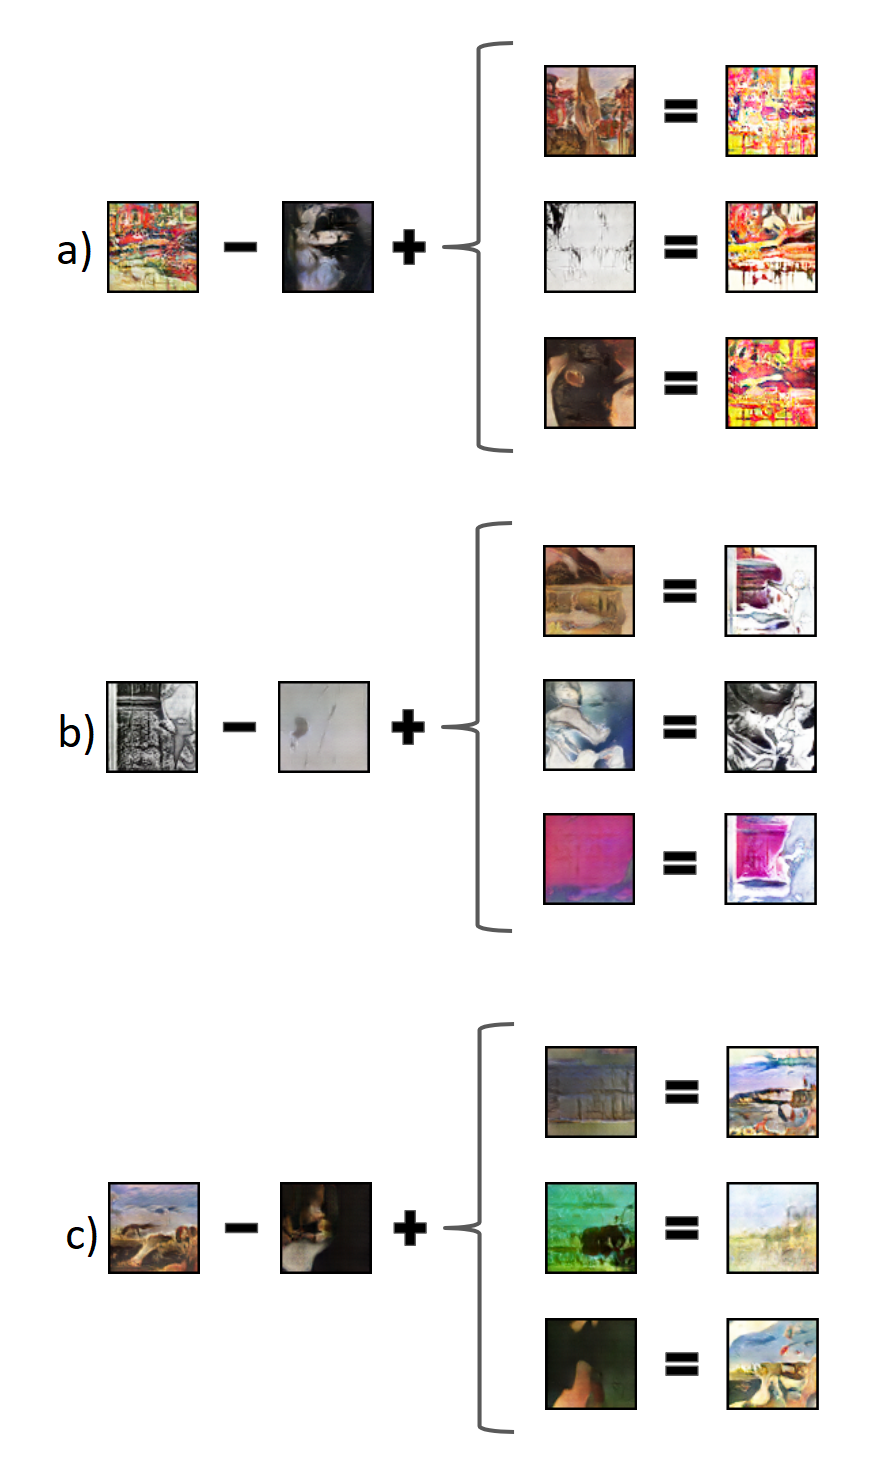
\includegraphics[width=0.8\linewidth]{arith_figure.png}
	\end{center}
	\caption{The results of our experiments with vector arithmetic in $ G $'s input space. Vector arithmetic does appear to preserve some properties of $ G(z_1) $ and $ G(z_3) $, but the effects are largely unpredictable.}
	\label{fig:long}
	\label{fig:onecol}
\end{figure}

\begin{figure}[t]
	\begin{center}
		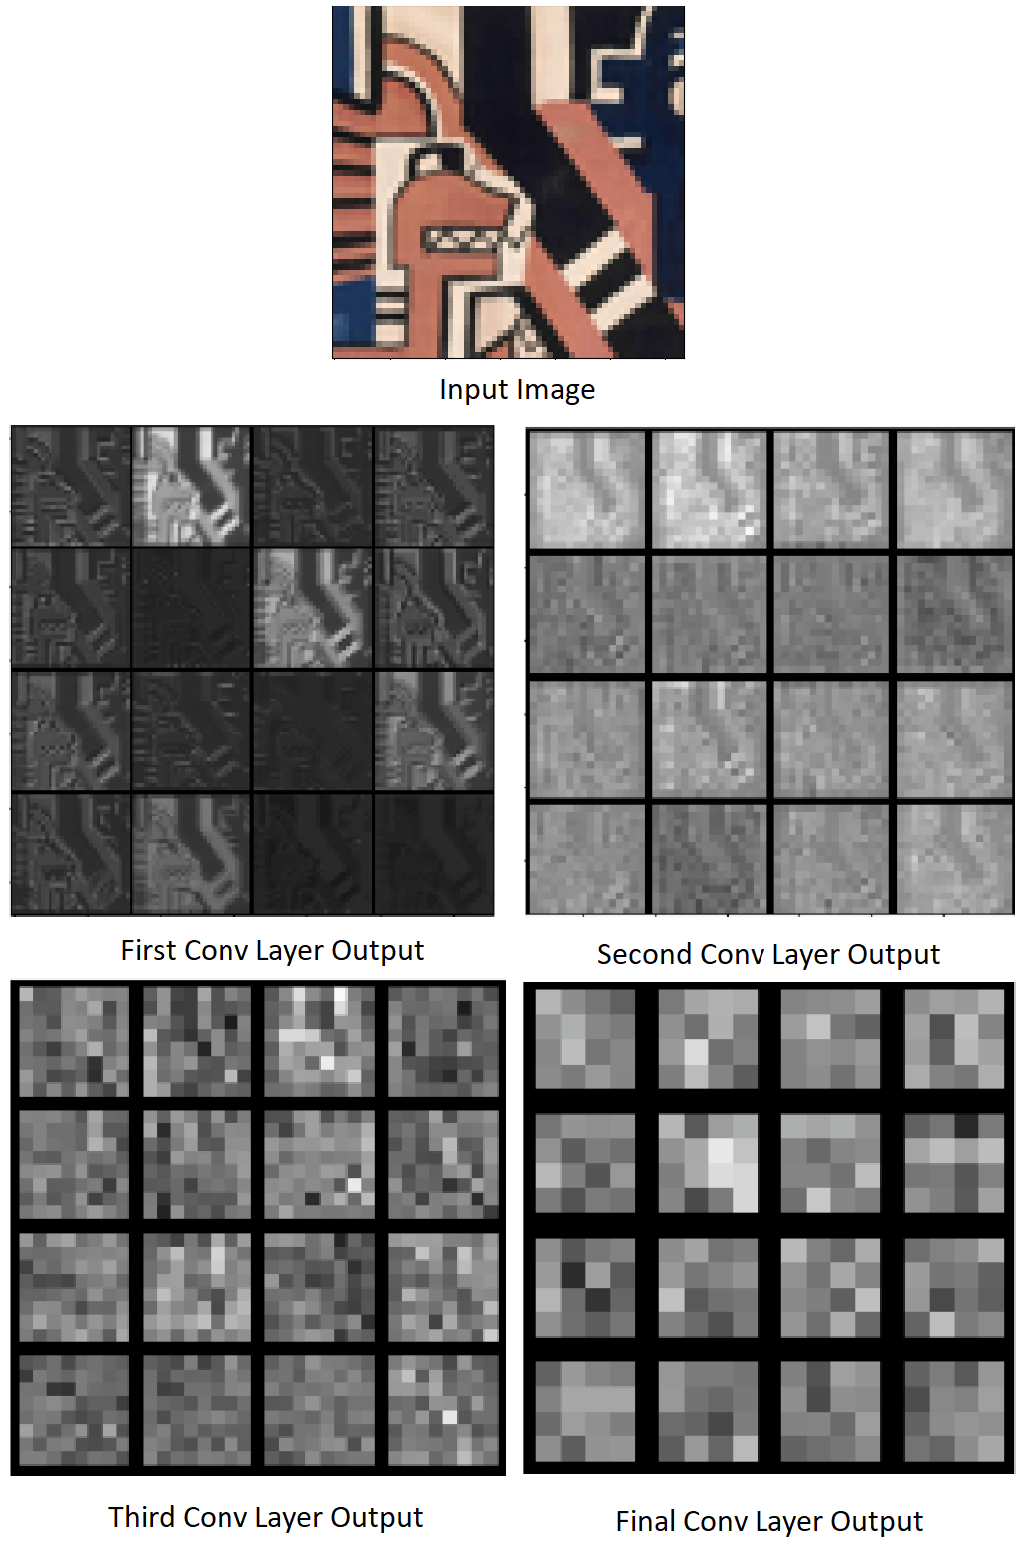
\includegraphics[width=0.675\linewidth]{deconv_full.png}
	\end{center}
	\caption{Output from a 'deconvnet' which reverses $ D $'s architecture to produce visualizations of the activations induced by passing the input image forward through $ D $. Only 16 filters from each convolution layer are show, the actual number of filters is larger and increases in the deeper layers.}
	\label{fig:long}
	\label{fig:onecol}
\end{figure}

\section{Conclusion}
We implement a DCGAN to train a generative model that learns visual features reflective of those present in the painting dataset we gathered, despite the relatively limited image resolution. Paintings generated are visually pleasing and showcase variety in color, form, and composition. Clear distinctions of genre and style can be seen in images, displaying the network's ability to learn stylistically meaningful features and representations of how those features come together to form genres. We also directly investigate the representations learned by our models to show their structure and quality using a variety of techniques.

\subsection{Future Work}
Many opportunities exist for future expansion on this work. With a deeper, more complex model architecture, we could potentially train a generative model to produce much higher resolution images with more intricate detail. Additionally, the dataset is ripe with contextual information such as style, genre, and artist that we have not employed in our models. Attributes such as these could be used to train a conditional GAN \cite{mirza2014conditional} which could produce artwork in requested styles rather than at random. It is also possible that including this metadata in the training process could aid the discriminator and generator in learning specific features or objects associated with specific attributes.

Recently, advances have been made in neural networks which are able to form an association between visual and linguistic concepts \cite{ishibashi2018associative}. Most paintings in our dataset are labeled with their title, which could allow a properly structured network to learn an association between visual concepts in paintings to linguistic concepts in their titles. Painting titles may be an easier dataset to work with than sentence descriptors, as they are generally shorter than sentences and they are less likely to be obfuscated by complex grammar structures, or to have grammar structure at all. However, they can still provide contextual information by describing painting content, or by conveying a mood or emotion that relates to specific color balances, styles, or forms. While there have been successful GAN implementations for text generation \cite{zhang2017adversarial}, there have yet to be any that successfully incorporate both image and textual learning. It is also possible that the manner in which a GAN learns could enable this associative mapping to be learned more effectively than a recurrent neural network, as it builds up feature knowledge rather than extracting it from given information.

{\small
\bibliographystyle{ieee}
\bibliography{sbgan}
}

\end{document}
